% Created by tikzDevice version 0.10.1 on 2017-11-22 20:46:45
% !TEX encoding = UTF-8 Unicode
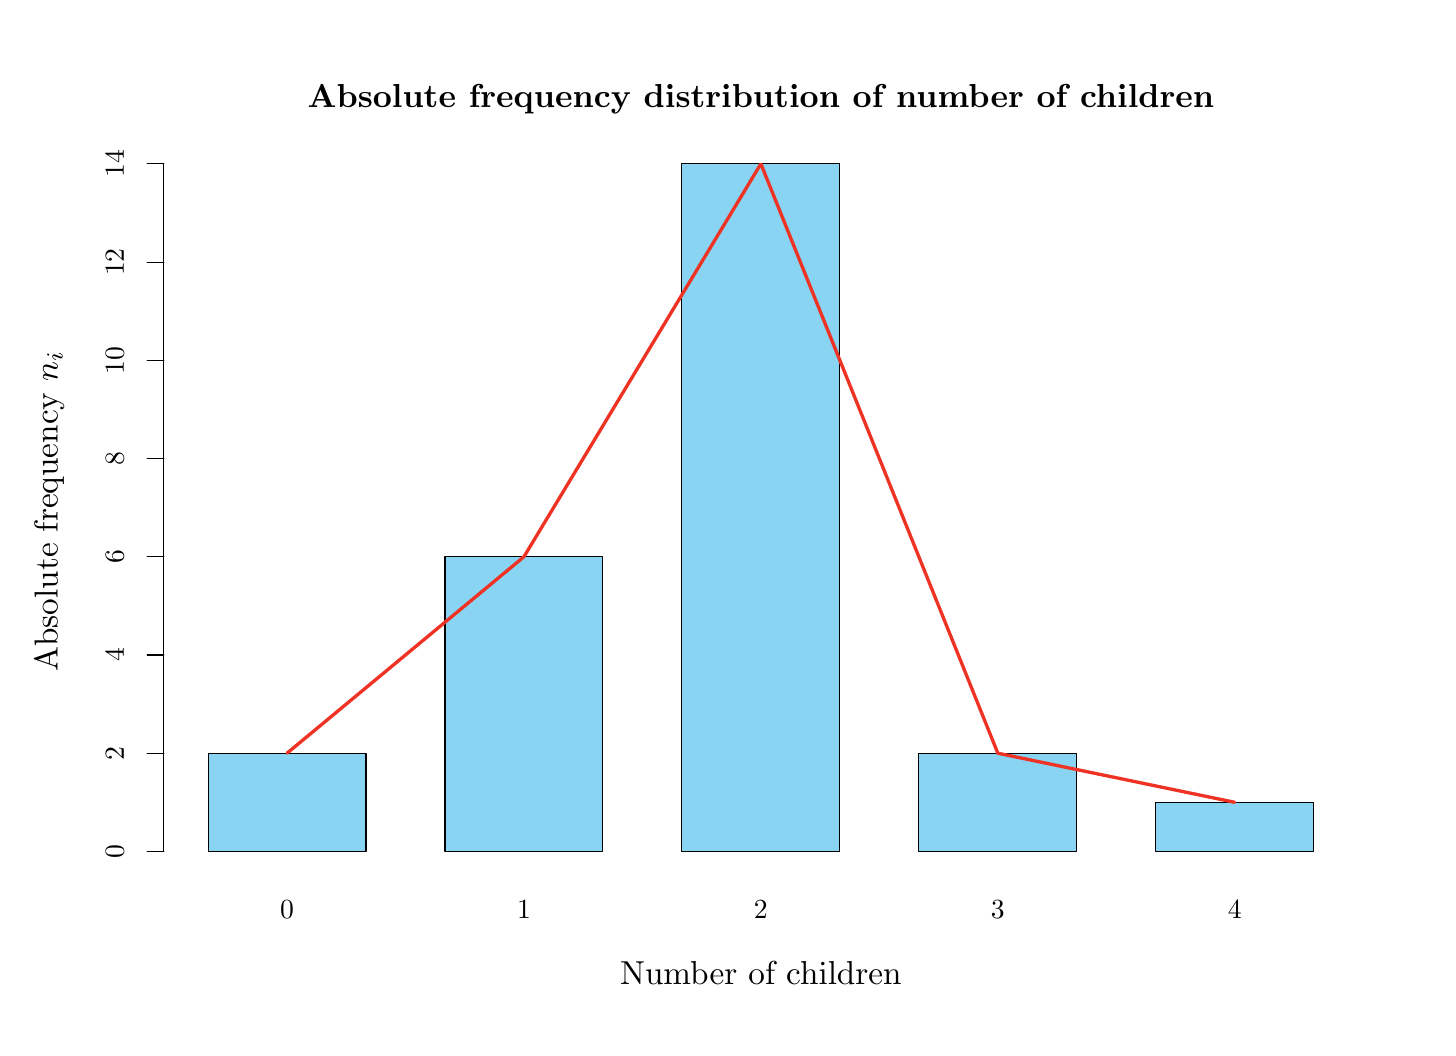
\begin{tikzpicture}[x=1pt,y=1pt]
\definecolor{fillColor}{RGB}{255,255,255}
\path[use as bounding box,fill=fillColor,fill opacity=0.00] (0,0) rectangle (505.89,361.35);
\begin{scope}
\path[clip] (  0.00,  0.00) rectangle (505.89,361.35);
\definecolor{drawColor}{RGB}{0,0,0}
\definecolor{fillColor}{RGB}{137,211,243}

\path[draw=drawColor,line width= 0.4pt,line join=round,line cap=round,fill=fillColor] ( 65.18, 63.68) rectangle (122.26, 99.18);

\path[draw=drawColor,line width= 0.4pt,line join=round,line cap=round,fill=fillColor] (150.79, 63.68) rectangle (207.87,170.17);

\path[draw=drawColor,line width= 0.4pt,line join=round,line cap=round,fill=fillColor] (236.41, 63.68) rectangle (293.48,312.15);

\path[draw=drawColor,line width= 0.4pt,line join=round,line cap=round,fill=fillColor] (322.02, 63.68) rectangle (379.10, 99.18);

\path[draw=drawColor,line width= 0.4pt,line join=round,line cap=round,fill=fillColor] (407.63, 63.68) rectangle (464.71, 81.43);
\end{scope}
\begin{scope}
\path[clip] (  0.00,  0.00) rectangle (505.89,361.35);
\definecolor{drawColor}{RGB}{0,0,0}

\node[text=drawColor,anchor=base,inner sep=0pt, outer sep=0pt, scale=  1.00] at ( 93.72, 39.60) {0};

\node[text=drawColor,anchor=base,inner sep=0pt, outer sep=0pt, scale=  1.00] at (179.33, 39.60) {1};

\node[text=drawColor,anchor=base,inner sep=0pt, outer sep=0pt, scale=  1.00] at (264.94, 39.60) {2};

\node[text=drawColor,anchor=base,inner sep=0pt, outer sep=0pt, scale=  1.00] at (350.56, 39.60) {3};

\node[text=drawColor,anchor=base,inner sep=0pt, outer sep=0pt, scale=  1.00] at (436.17, 39.60) {4};
\end{scope}
\begin{scope}
\path[clip] (  0.00,  0.00) rectangle (505.89,361.35);
\definecolor{drawColor}{RGB}{0,0,0}

\node[text=drawColor,anchor=base,inner sep=0pt, outer sep=0pt, scale=  1.20] at (264.94,332.61) {\bfseries Absolute frequency distribution of number of children};

\node[text=drawColor,anchor=base,inner sep=0pt, outer sep=0pt, scale=  1.20] at (264.94, 15.60) {Number of children};

\node[text=drawColor,rotate= 90.00,anchor=base,inner sep=0pt, outer sep=0pt, scale=  1.20] at ( 10.80,186.67) {Absolute frequency $n_i$};
\end{scope}
\begin{scope}
\path[clip] (  0.00,  0.00) rectangle (505.89,361.35);
\definecolor{drawColor}{RGB}{0,0,0}

\path[draw=drawColor,line width= 0.4pt,line join=round,line cap=round] ( 49.20, 63.68) -- ( 49.20,312.15);

\path[draw=drawColor,line width= 0.4pt,line join=round,line cap=round] ( 49.20, 63.68) -- ( 43.20, 63.68);

\path[draw=drawColor,line width= 0.4pt,line join=round,line cap=round] ( 49.20, 99.18) -- ( 43.20, 99.18);

\path[draw=drawColor,line width= 0.4pt,line join=round,line cap=round] ( 49.20,134.67) -- ( 43.20,134.67);

\path[draw=drawColor,line width= 0.4pt,line join=round,line cap=round] ( 49.20,170.17) -- ( 43.20,170.17);

\path[draw=drawColor,line width= 0.4pt,line join=round,line cap=round] ( 49.20,205.66) -- ( 43.20,205.66);

\path[draw=drawColor,line width= 0.4pt,line join=round,line cap=round] ( 49.20,241.16) -- ( 43.20,241.16);

\path[draw=drawColor,line width= 0.4pt,line join=round,line cap=round] ( 49.20,276.65) -- ( 43.20,276.65);

\path[draw=drawColor,line width= 0.4pt,line join=round,line cap=round] ( 49.20,312.15) -- ( 43.20,312.15);

\node[text=drawColor,rotate= 90.00,anchor=base,inner sep=0pt, outer sep=0pt, scale=  1.00] at ( 34.80, 63.68) {0};

\node[text=drawColor,rotate= 90.00,anchor=base,inner sep=0pt, outer sep=0pt, scale=  1.00] at ( 34.80, 99.18) {2};

\node[text=drawColor,rotate= 90.00,anchor=base,inner sep=0pt, outer sep=0pt, scale=  1.00] at ( 34.80,134.67) {4};

\node[text=drawColor,rotate= 90.00,anchor=base,inner sep=0pt, outer sep=0pt, scale=  1.00] at ( 34.80,170.17) {6};

\node[text=drawColor,rotate= 90.00,anchor=base,inner sep=0pt, outer sep=0pt, scale=  1.00] at ( 34.80,205.66) {8};

\node[text=drawColor,rotate= 90.00,anchor=base,inner sep=0pt, outer sep=0pt, scale=  1.00] at ( 34.80,241.16) {10};

\node[text=drawColor,rotate= 90.00,anchor=base,inner sep=0pt, outer sep=0pt, scale=  1.00] at ( 34.80,276.65) {12};

\node[text=drawColor,rotate= 90.00,anchor=base,inner sep=0pt, outer sep=0pt, scale=  1.00] at ( 34.80,312.15) {14};
\end{scope}
\begin{scope}
\path[clip] ( 49.20, 61.20) rectangle (480.69,312.15);
\definecolor{drawColor}{RGB}{238,50,36}

\path[draw=drawColor,line width= 1.2pt,line join=round,line cap=round] ( 93.72, 99.18) --
	(179.33,170.17) --
	(264.94,312.15) --
	(350.56, 99.18) --
	(436.17, 81.43);
\end{scope}
\end{tikzpicture}
